
	Es importante recalcar que la ganancia de Kalman $K_k$ es distinta para cada instante $k$. Cuando el sistema es variante en el tiempo, el filtro se adapta a las condiciones de dinámica y ruido instante a instante. En el caso contrario, cuando el sistema es invariante en el tiempo, puede demostrarse que tanto la matriz $K_k$, como la matriz $P_k$, convergen para tiempo infinito. Es decir:


	\begin{equation*}
		K_k \longrightarrow K
	\end{equation*}
	
	\begin{equation*}
		P_k \longrightarrow P
	\end{equation*}
	
	para $k \rightarrow \infty$. Dichas matrices pueden computarse mediante ecuaciones aritméticas discretas de Riccati (\emph{DARE}). Es decir, $P$ debe cumplir:
	
	\begin{equation*}
		P = A P A^{*} - A P C^{*} (R + C P C^{*})^{-1} C P A + B Q B^{*}
	\end{equation*}
	
	Por otro lado la ganancia de Kalman puede calcularse como:
	
	\begin{equation*}
		K = P C^{*} (R + C P C^{*})^{-1}
	\end{equation*}
	
	Dadas estas matrices, surge la posibilidad de implementar una modificación al algoritmo de Kalman para que en lugar de utilizar las matrices calculadas instante a instante siempre utilice las matrices a las que va a converger, suponiendo que el sistema es invariante en el tiempo. Dicho algoritmo tiene la ventaja de que posee menos procesamiento en tiempo real, dado que las matrices $K$ y $P$ pueden computarse en tiempo de compilación y guardarse fijas en la memoria. Este algoritmo no será óptimo, pero puede demostrarse que la versión modificada convergerá a la versión original con rapidez exponencial, siendo más los beneficios que trae que los inconvenientes. El objetivo de este punto es comparar las dos variantes y demostrar lo expuesto. En la Figura \ref{fig:ej3f_cov} se puede ver el resultado de la estimación. En línea punteada azul puede verse que la estimación del algoritmo modificado comienza desviada de la trayectoria, pero rápidamente converge a la misma. 

	\begin{figure}[H]
		\centering
		%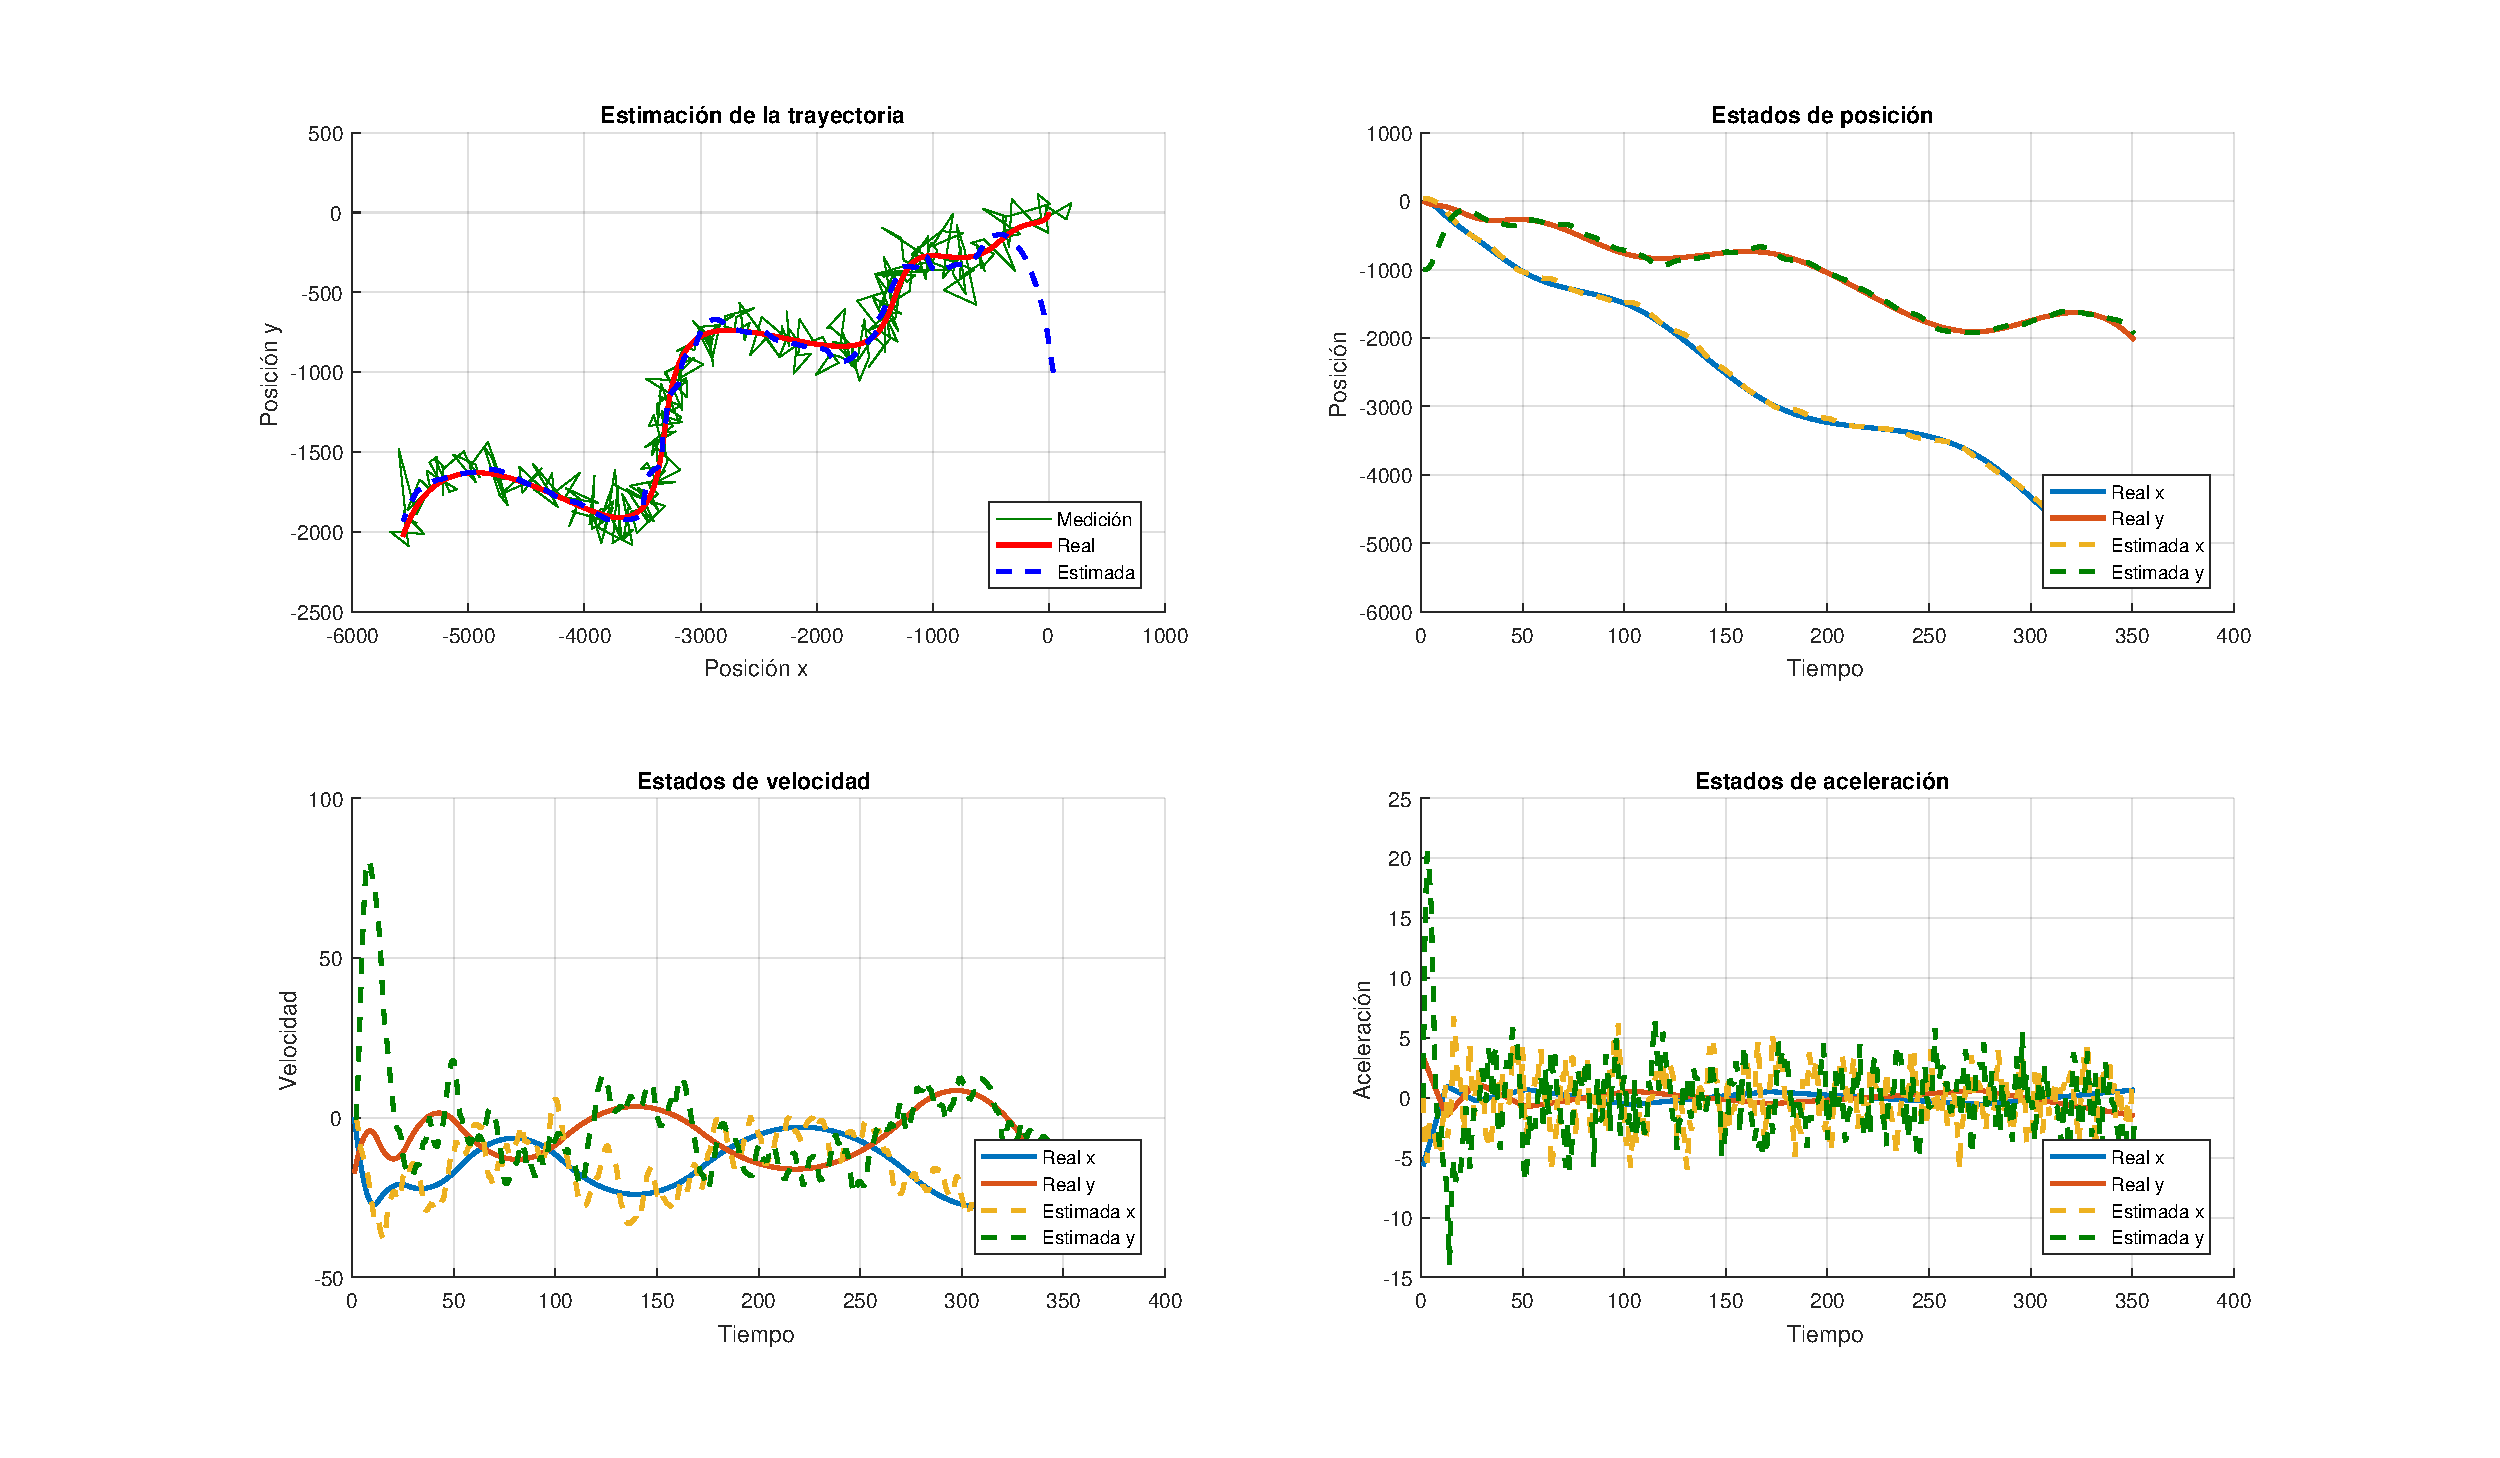
\includegraphics[width=1.0\textwidth,keepaspectratio]{Figuras/graf_ej5.pdf}
		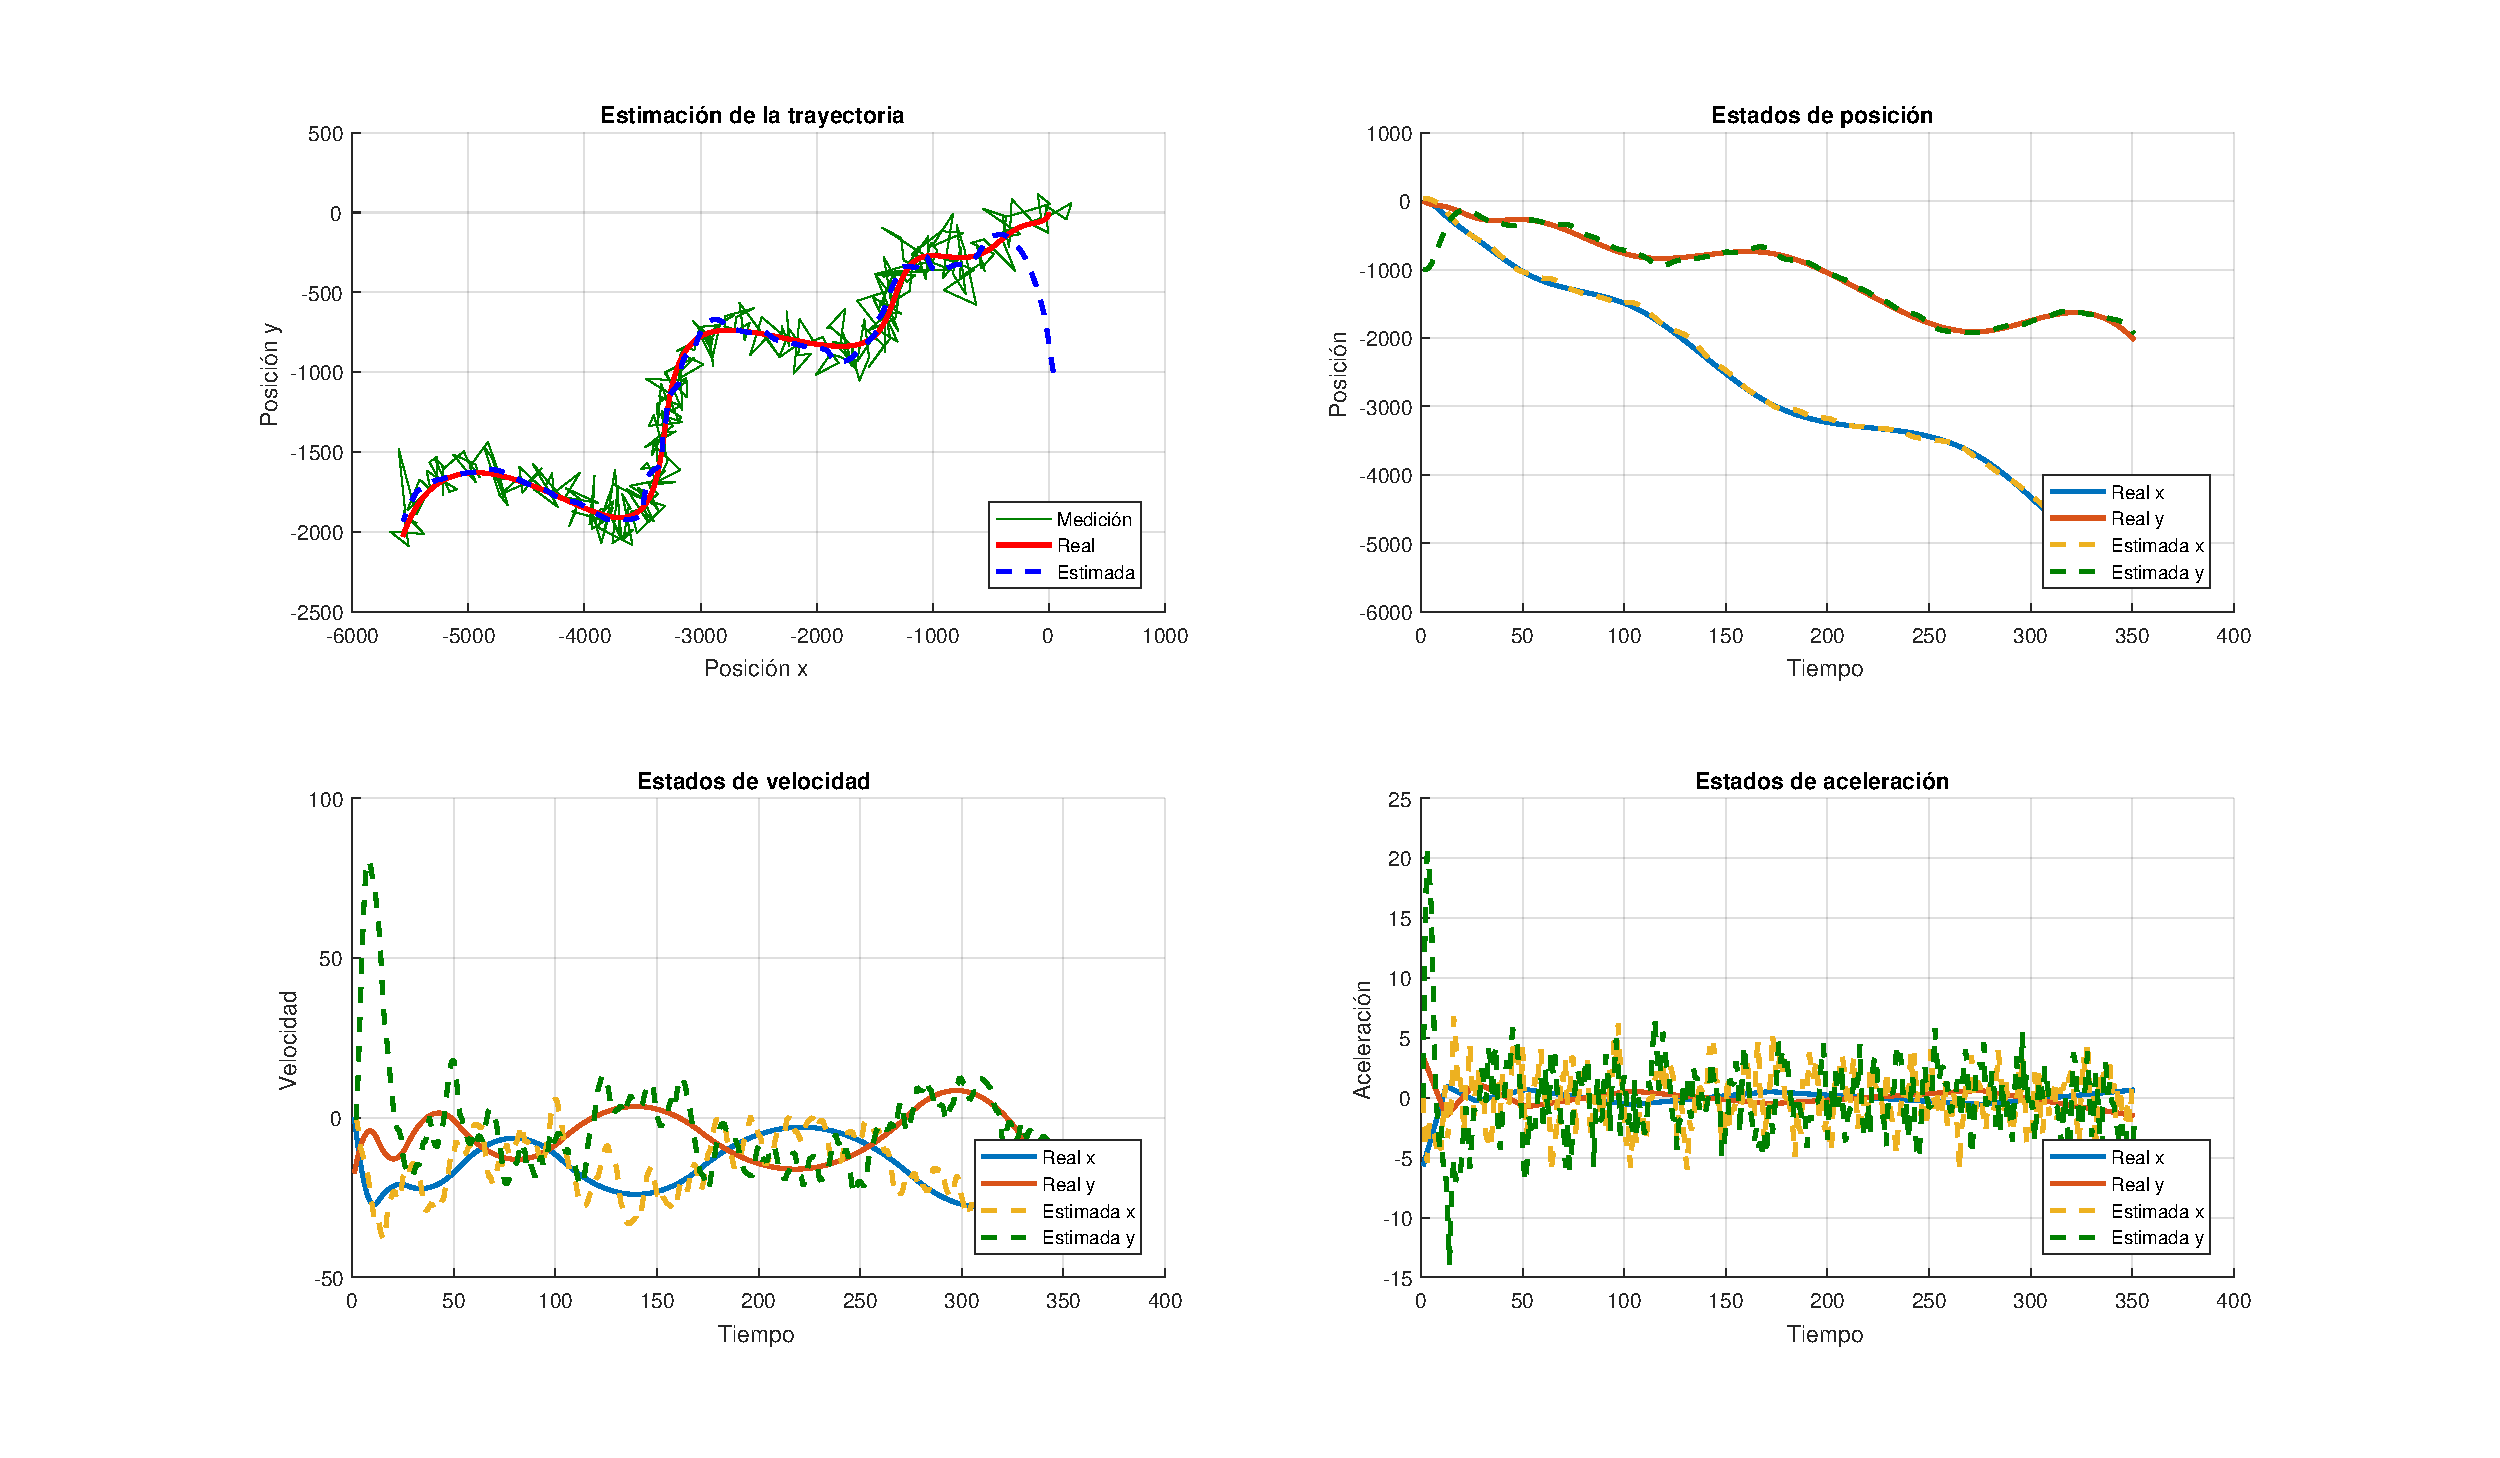
\includegraphics[scale=0.5,trim={6,5cm 0 0 0}]{Figuras/graf_ej5.pdf}
		\caption{Estimación de Trayectoria}
		\label{fig:ej5}
	\end{figure}
	
	Se puede ver también que la correlación de las innovaciones no corresponde totalmente al de un proceso blanco y por tanto podría justificarse que es un factor por el cual difiere el Kalman estacionario del original.
	\begin{figure}[H]
		\centering
		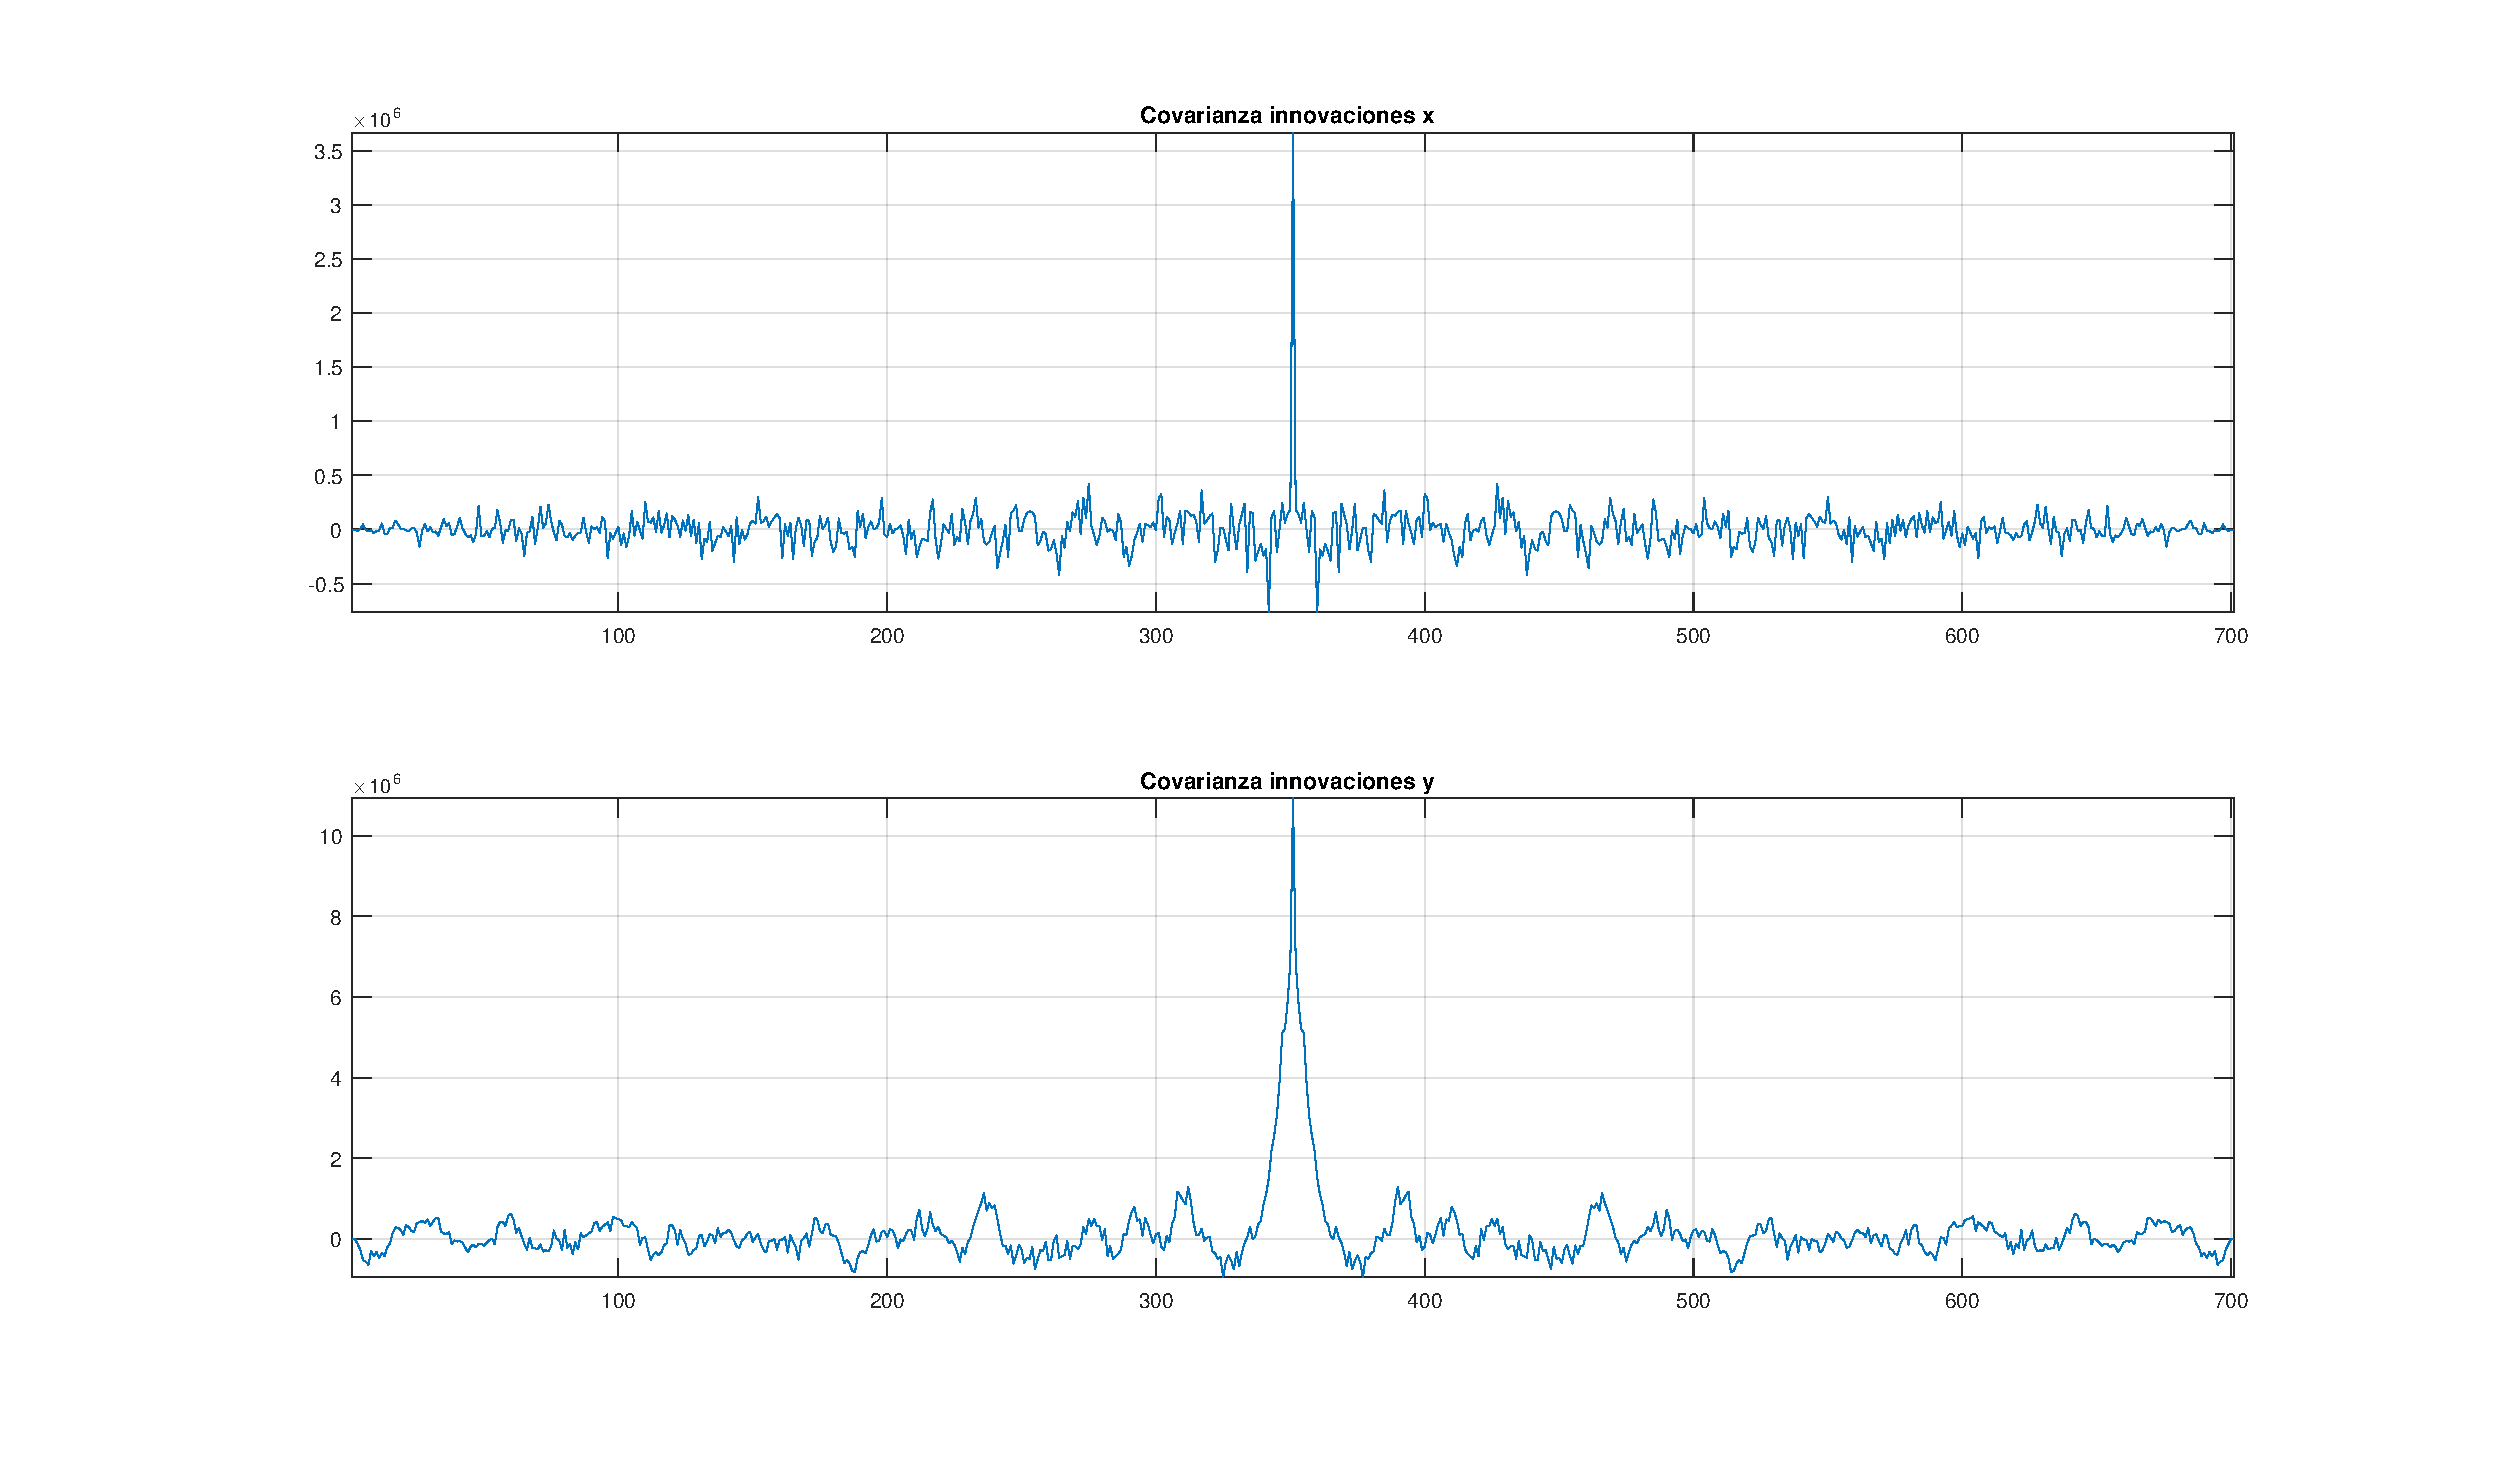
\includegraphics[width=1.0\textwidth,keepaspectratio]{Figuras/covinn_ej5.pdf}
		\caption{Correlación De Innovaciones}
		\label{fig:ej6_cov}
	\end{figure}

	A continuación se exponen las matrices $P$ y $K$ de los Kalman modificado y el original en estado estacionario.
	\begin{equation}
	P_{\textit{DARE}} = \begin{bmatrix} \num{2.821}&0&\num{10.85}&0&22.74&0 \\[0.3em] 0&\num{28.21}&0&\num{10.85}&0&\num{22.74}\\[0.3em] \num{10.85}&0&\num{74.91}&0&\num{191.2}&0\\[0.3em] 0&\num{10.85}&0&\num{74.91}&0&\num{191.2}\\[0.3em] \num{22.74}&0&\num{191.2}&0&\num{728.3}&0\\[0.3em] 0&\num{22.74}&0&\num{191.2}&0&\num{728.3}\end{bmatrix}\times\num{e-3}
		\label{eq:pdare}
	\end{equation}

	\begin{equation}
	K_{\textit{DARE}} = \begin{bmatrix} \num{0.2521}&0&\num{1.085}&0&\num{2.274}&0\\[0.3em] 0&\num{.2521}&0&\num{1.085}&0&\num{2.274}\\[0.3em] \num{83.33}&0&\num{620.6}&0&\num{1685}&0\\[0.3em] 0&\num{83.33}&0&\num{620.6}&0&\num{1685}\\[0.3em] \num{13150}&0&\num{123700}&0&\num{538400}&0\\[0.3em] 0&\num{13150}&0&\num{123700}&0&\num{538400}\end{bmatrix}\times\num{e-6}
		\label{eq:kdare}
	\end{equation}

	\begin{equation}
	P_{k/k} = \begin{bmatrix}\num{17.18}&0&\num{3.355}&0&\num{0.3489}0\\[0.3em] 0&\num{17.18}&0&\num{3.355}&0&\num{0.3489}\\[0.3em] \num{-3.356}&0&\num{-0.3479}&0&\num{-22.90e-3}&0\\[0.3em]0&\num{-3.356}&0&\num{-0.3479}&0&\num{-22.90e-3}\\[0.3em] \num{0.3498}&0&\num{-0.001963}&0&\num{0.046012e-3}&0\\[0.3em] 0&\num{0.3498}&0&\num{-0.001963}&0&\num{0.046012e-3}\\[0.3em]\end{bmatrix}
		\label{eq:pk}
	\end{equation}

	\begin{equation}
	K_k = \begin{bmatrix} \num{0.001715}&0&\num{0.03361}&0&\num{0.3448}&0\\[0.3em] 0&\num{0.001715}&0&\num{0.03361}&0&\num{0.3448}\\[0.3em] \num{-0.0003362}&0&\num{-0.003480}&0&\num{0.0001391}&0\\[0.3em] 0&\num{-0.0003362}&0&\num{-0.003480}&0&\num{0.0001391}\\[0.3em] \num{0.00003437}&0&\num{-0.00002020}&0&\num{0.009934}&0\\[0.3em] 0&\num{0.00003437}&0&\num{-0.00002020}&0&\num{0.009934}\\[0.3em] \end{bmatrix}
		\label{eq:kk}
	\end{equation}

	Se puede apreciar que las matrices de las Ecuaciones \eqref{eq:pdare} y \eqref{eq:pk} distan de ser semejantes como también sucede con \eqref{eq:kdare} y \eqref{eq:kk}. Ésta puede ser la razón por la cual la aceleración estimada (Figura \ref{fig:ej5}) difiere mucho del valor real.
	

